\documentclass[tikz,border=3mm]{standalone}
\begin{document}

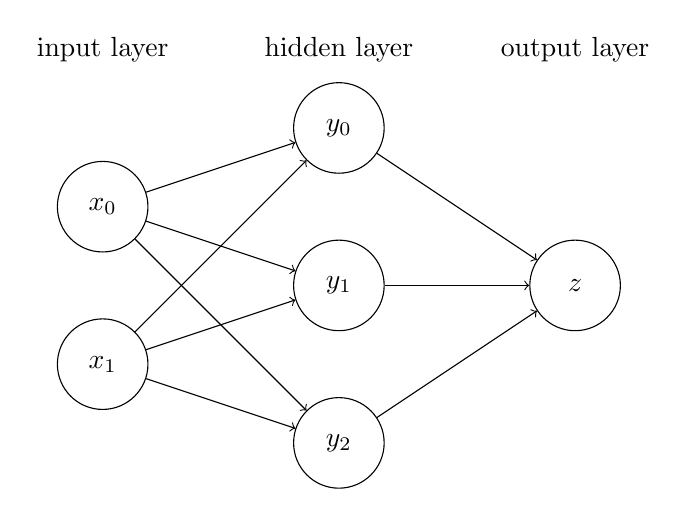
\begin{tikzpicture}
	\tikzstyle{unit}=[draw,shape=circle,minimum size=1.15cm]
	%\tikzstyle{hidden}=[draw,shape=circle,fill=black!25,minimum size=1.15cm]
	\tikzstyle{hidden}=[draw,shape=circle,minimum size=1.15cm]

	\node[unit](x0) at (0,2){$x_0$};
	\node[unit](x1) at (0,0){$x_1$};
	\node[unit](y0) at (3,3){$y_0$};
	\node[unit](y1) at (3,1){$y_1$};
	\node[unit](y2) at (3,-1){$y_2$};
		
	\node[unit](z) at (6,1){$z$};

	\draw[->] (x0) -- (y0);
	\draw[->] (x0) -- (y1);
    \draw[->] (x0) -- (y2);

	\draw[->] (x1) -- (y0);
	\draw[->] (x1) -- (y1);
    \draw[->] (x1) -- (y2);

	\draw[->] (y0) -- (z);
	\draw[->] (y1) -- (z);
	\draw[->] (y2) -- (z);
	
	\draw (0,4) node {input layer};
	\draw (3,4) node {hidden layer};
	\draw (6,4) node {output layer};
\end{tikzpicture}

\end{document}